\documentclass[12pt,a4paper]{article}
% Языки, которые могут быть использованы.
\usepackage[english,russian]{babel}

% FreeSerif — альтернатива TimesNewRoman
\usepackage{fontspec}
\setmainfont[Ligatures=TeX]{Times New Roman}
\setmonofont[Mapping=,Ligatures=]{Courier New}

% Чтобы сделать буковки ещё красивее.
\usepackage{microtype}

% Картинки, вращение и всё такое. Причём даже в режиме черновика
\usepackage[final]{graphicx}
\usepackage{float}
\usepackage[draft=no]{svg}
\usepackage{pdfpages}

% Чтобы легко менять стиль списков
\usepackage[shortlabels]{enumitem}

\usepackage{unicode-math}
\usepackage{csquotes}
\usepackage{adjustbox}
\usepackage{relsize}

% https://tex.stackexchange.com/questions/14967/source-code-listing-with-frame-around-code
\usepackage{listings}
\lstset{frame=lrbt,xleftmargin=\fboxsep,xrightmargin=-\fboxsep}
\lstset{basicstyle=\ttfamily,breaklines=true}

% https://qna.habr.com/answer?answer_id=1140867
\bibliographystyle{gost2008}
\usepackage[
	style=gost-numeric, % стиль цитирования и библиографии, см. документацию biblatex-gost
	language=auto,  % использовать язык из babel
	autolang=other, % многоязычная библиография
	parentracker=true,
	backend=biber,
	hyperref=true,
	bibencoding=utf8,
	sorting=ntvy,  % сортировка: имя, заголовок, том, год
]{biblatex}
\addbibresource{bibliography.bib}
\DeclareSourcemap{
    \maps{
        \map{% если @online, то устанавливаем media=eresource.
            \step[typesource=online, fieldset=media, fieldvalue=eresource]
        }
    }
}

% Отсупы как по госту.
\usepackage[
	includeheadfoot,
	left=20mm,
	right=10mm,
	top=0mm,
	headheight=25mm,
	footskip=5\baselineskip, % footskip is the distance between the textbody and the baseline of the footer
	bottom=15mm,
]{geometry}

\savegeometry{original}
\geometry{bottom=10mm}
\savegeometry{nofooter}
\loadgeometry{original}

%% Некоторые переменные, которые появляются более одного раза

% Название курсовой. Не забывать проценты в конце строк.
\newcommand{\docTitle}{%
	Сервис для индексирования и просмотра репозиториев%
}

\newcommand{\docTitleEng}{%
	Repository Indexing and Viewing Service%
}

% Год написания курсовой.
\newcommand{\YEAR}{
	\the\year{}
}

% RU — код страны
% 17701729 — код НИУ ВШЭ
% 05.15 — регистрационный номер (https://docs.cntd.ru/document/566085681)
% 		В данном случае, Прикладное ПО / Информационные системы для решения специфических отраслевых задач
% 01 — номер редакции документа
% 33 — код вида документа (https://www.swrit.ru/doc/espd/19.101-77.pdf#page=4)
% 01 — номер документа данного вида
%  1 — номер части документа
\newcommand{\docId}{RU.17701729.03.10-01 12 01-1}


% Footer and header
\usepackage{fancyhdr}
\pagestyle{fancy}
\fancyhf{}
\chead{
	%\bf % Сделать жирненьким
	\thepage\\
	\docId
}
\fancyhead[RO]{%
    % В правый верхний колотитул пихаю номер приложения
    {\ifnum\value{addendum}>0 ПРИЛОЖЕНИЕ \theaddendum \fi}
}
\cfoot{%
	\adjustbox{valign=b}{ % baseline of footer at bottom, so margins are correct
		\begin{tabular}{| l | l | l | l | l |}
			\hline & & & & \\
			\hline Изм. & Лист & № докум. & Подп. & Дата \\
			\hline \docId &  &  &  &  \\
			\hline Инв. № подл. & Подп. и дата & Взам. инв. № & Инв. № дубл. & Подп. и дата № \\
			\hline
		\end{tabular}
	}
}
\fancypagestyle{nofooter}{%
	\fancyfoot{}%
}

\renewcommand{\headrulewidth}{0pt}
\renewcommand{\footrulewidth}{0pt}

% Повернуть на 90 градусов
\newcommand{\rot}[2]{\rotatebox[origin=c]{90}{\enspace\parbox{#1 - 0.5em}{#2}}}

% Повторить #1 раз текст #2: \Repeat{#1}{#2}
\usepackage{expl3}
\ExplSyntaxOn
\cs_new_eq:NN \Repeat \prg_replicate:nn
\ExplSyntaxOff

% Продвинутые таблицы
\usepackage{tabularx}
\usepackage{multirow}
\usepackage{xltabular}
% И сразу делаем чтобы колонки X центрировались по вертикали
\def\tabularxcolumn#1{m{#1}}
\newcolumntype{Y}{>{\centering\arraybackslash}X}

% Подсчет числа страниц
\usepackage{lastpage}

% Расчет всяких размеров
\usepackage{calc}

% Названия разделов по центру (но titlesec конфликтует с hyperref)
\usepackage{titlesec}
\titleformat{\section}
  {\centering\Large\bfseries}
  {\thesection}
  {.5em}
  {\MakeUppercase}
% И с точкой в конце.
\titlelabel{\thetitle.\quad}

% После названия раздела надо делать отступы у абзацев.
\usepackage{indentfirst}

% https://tex.stackexchange.com/a/347803
\usepackage{varwidth}

\newcommand{\placename}{
	\underline{\hspace{4cm}}
}
\newcommand{\placedate}{
	«\underline{\hspace{1em}}» \underline{\hspace{3cm}} \YEAR г.
}

\newcounter{addendum}
\makeatletter
\newcommand{\addendum}[1]{
    \stepcounter{addendum}

	% Приложения есть в оглавлении
	\phantomsection
	\addcontentsline{toc}{section}{Приложение \arabic{addendum}: #1}

	\section*{#1}
	
	% Сбросить все счетчики
	\setcounter{equation}{0}
    \setcounter{figure}{0}
    \setcounter{table}{0}

	% Треш и угар с макросами, чтобы обойти проблемы между titlsec и hyperref
	% Цель: \NR@gettitle{Приложение 1: …}, но нужно **сначала** раскрыть \arabic{addendum}
	\edef\addendumTitle{\noexpand\NR@gettitle{Приложение \arabic{addendum}: #1}}
	\addendumTitle
}
\makeatother

% Ещё больше подсекций
\newcommand{\subsubsubsection}[1]{\paragraph{#1}\mbox{}\\}
\setcounter{secnumdepth}{4}
\setcounter{tocdepth}{4}

% TODOшечки
\usepackage{ifdraft}
\ifdraft{
	% Если \document[draft], то нам нужно место в полях для todo.
	\geometry{left=40mm, right=5mm, marginparwidth=35mm}
	\reversemarginpar  % причём слева они выглядят симпатичнее
	\savegeometry{original}
}{}
\usepackage[obeyDraft,textsize=footnotesize,textwidth=35mm]{todonotes}

% Добавляем гипертекстовое оглавление в PDF
% hyperref должен быть последним
\usepackage[hidelinks]{hyperref}

\begin{document}
	\selectlanguage{russian}

	\newenvironment{LeftTablePage}{%
	\thispagestyle{empty}%
	% Временно уменьшаем отступы.
	\newgeometry{left=5mm, top=25mm, bottom=10mm}%
	% Содержимое слева.
	\noindent\begin{minipage}[b]{20mm}
		\rotatebox{90}{
			\begin{tabular}{| c | c | c | c | c |}
				\hline
				Инв. № подл. & Подп. и дата & Взам. инв. № & Инв. № дубл. & Подп. и дата \\
				\hline
				\docId & & & & \\
				\hline
			\end{tabular}%
		}
	\end{minipage}%
	% Основное содержимое
	\begin{samepage}%
	\begin{minipage}[b][\textheight]{\textwidth}\centering%
}{
	\end{minipage}%
	\end{samepage}
	
	% Теперь можно вернуть отступы как были
	\restoregeometry

	\clearpage
}

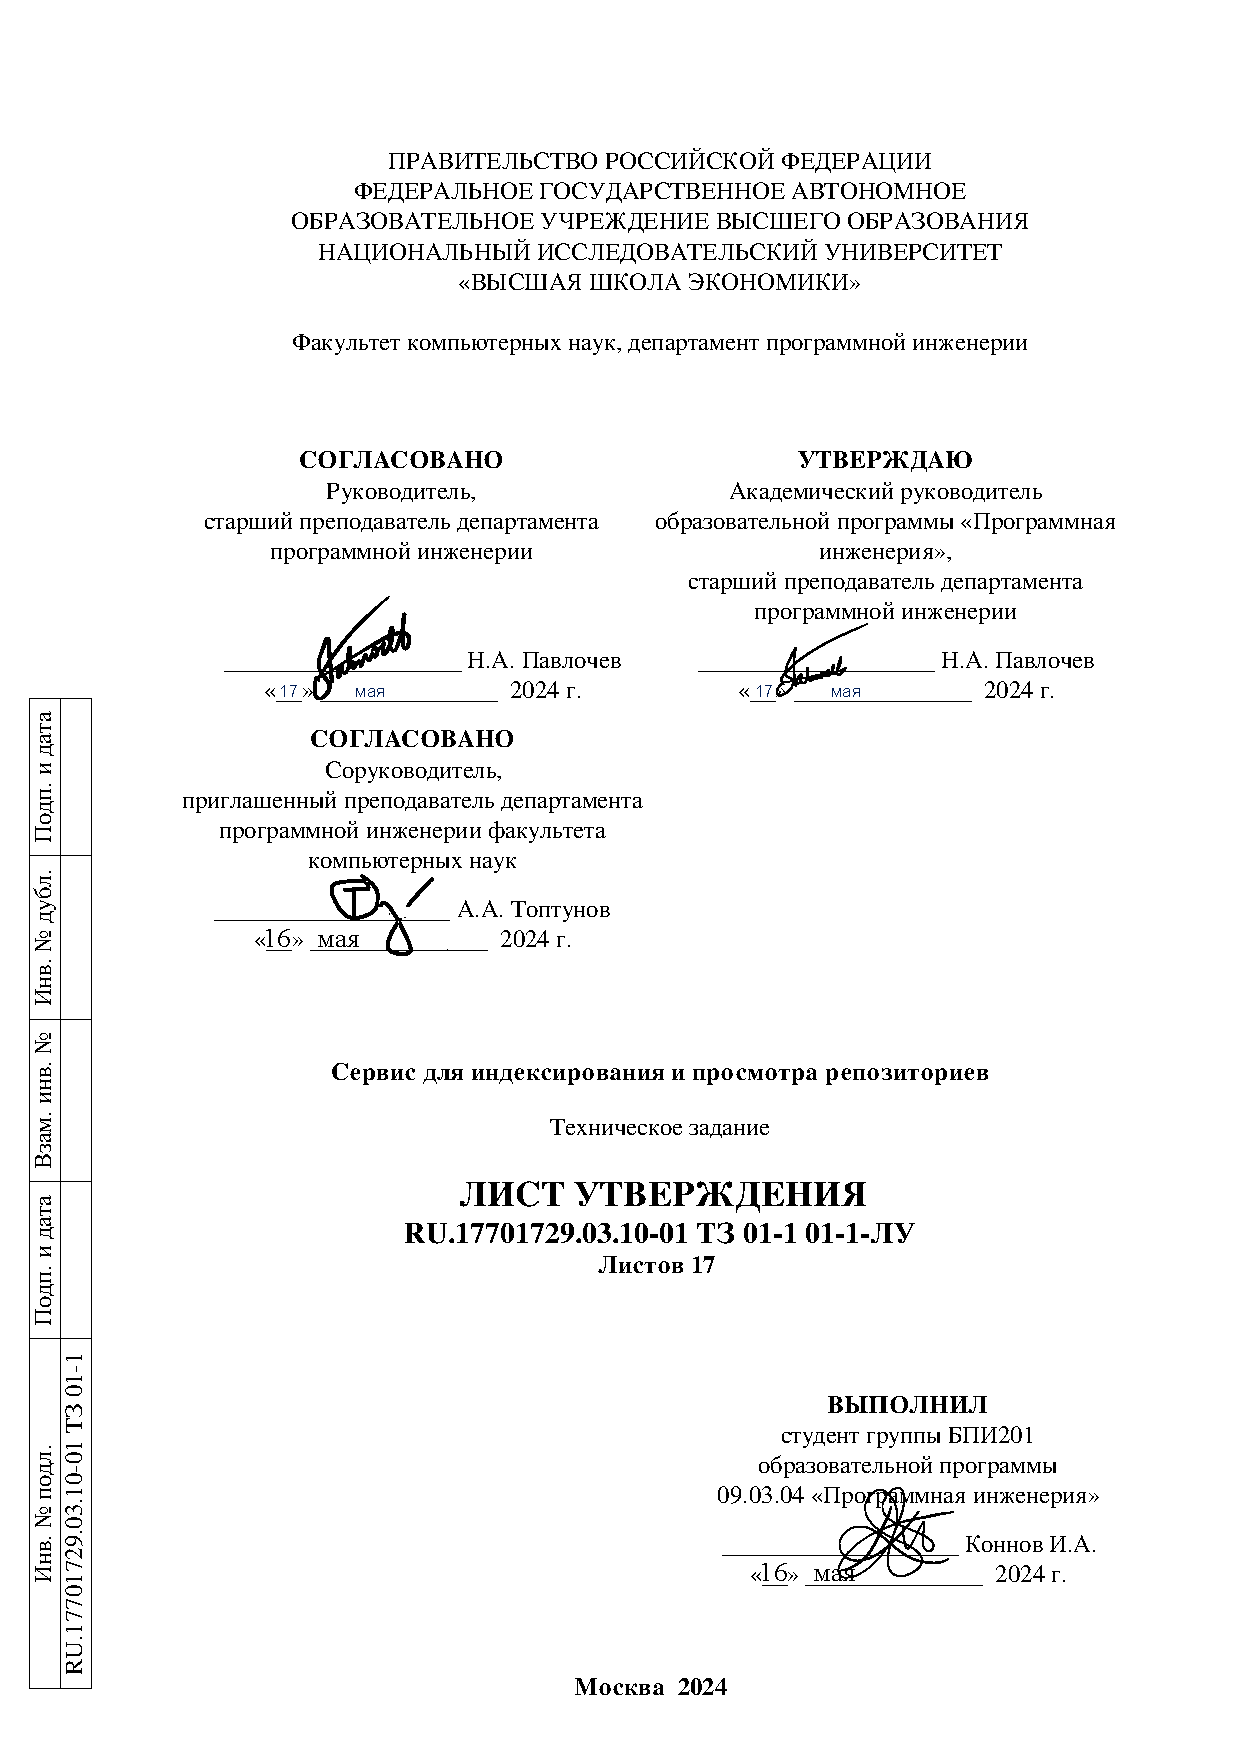
\includepdf[pages=-]{figures/signed.pdf}
% \begin{LeftTablePage}
% 	%% Лист утверждения
    ПРАВИТЕЛЬСТВО РОССИЙСКОЙ ФЕДЕРАЦИИ \\
    ФЕДЕРАЛЬНОЕ ГОСУДАРСТВЕННОЕ АВТОНОМНОЕ \\
    ОБРАЗОВАТЕЛЬНОЕ УЧРЕЖДЕНИЕ ВЫСШЕГО ОБРАЗОВАНИЯ \\
    НАЦИОНАЛЬНЫЙ ИССЛЕДОВАТЕЛЬСКИЙ УНИВЕРСИТЕТ \\
    «ВЫСШАЯ ШКОЛА ЭКОНОМИКИ» \\[1\baselineskip]
    Факультет компьютерных наук, департамент программной инженерии
\vskip 1.5cm
    % Согласовано / утверждаю
    \begin{varwidth}[t]{0.45\textwidth}\centering
    	\textbf{СОГЛАСОВАНО}
    	
    	Руководитель, \\
    	старший преподаватель департамента
        программной инженерии
    \end{varwidth}%
    \hfil%
    \begin{varwidth}[t]{0.45\textwidth}\centering
    	\textbf{УТВЕРЖДАЮ}
    	
    	Академический руководитель
        образовательной программы
        «Программная инженерия», \\
        старший преподаватель департамента
        программной инженерии
    \end{varwidth}

\bigskip

    \begin{varwidth}[t]{0.4\textwidth}\centering
    	\placename Н.А. Павлочев \\
    	\placedate
    \end{varwidth}%
    \hfil%
    \begin{varwidth}[t]{0.4\textwidth}\centering
    	\placename Н.А. Павлочев \\
    	\placedate
    \end{varwidth}

\bigskip

    \begin{minipage}[t]{0.45\textwidth}\centering
    	\textbf{СОГЛАСОВАНО}
    	
    	Соруководитель, \\
    	приглашенный преподаватель
        департамента программной инженерии
        факультета компьютерных наук
    \end{minipage}%
    \hfil\makebox[0.45\textwidth]{}

\bigskip

    \begin{minipage}[t]{0.45\textwidth}\centering
    	\placename А.А. Топтунов \\
    	\placedate
    \end{minipage}%
    \hfil\makebox[0.45\textwidth]{}

\vfill

    \textbf{\uppercase{\docTitle}}

    \bigskip

    Программа и методика испытаний

    \bigskip

    \textbf{
    	\Large
    		ЛИСТ УТВЕРЖДЕНИЯ \\
    	\large
    		{\docId} 01-1-ЛУ \\
    	\normalsize
    		Листов \pageref*{LastPage}
    }

\vfill

    \makebox[0.45\textwidth]{}\hfil%
    \begin{minipage}[t]{0.45\textwidth}\centering
    	\textbf{ВЫПОЛНИЛ}
            
    	студент группы БПИ201 \\
    	образовательной программы \\
    	09.03.04 «Программная инженерия» \\
    \end{minipage}

\bigskip

    \makebox[0.45\textwidth]{}\hfil%
    \begin{minipage}[t]{0.45\textwidth}\centering
    	\placename Коннов И.А. \\
    	\placedate
    \end{minipage}

\vskip 1.5cm

    \textbf{Москва \YEAR}
% \end{LeftTablePage}

% ГОСТ гласит, что лист утверждения не должен быть нумероваться: титульный лист это первый лист
\pagenumbering{arabic}

\begin{LeftTablePage}
	%% Первые две страницы ТЗ:
%% 1. Лист утверждения
%% 2. Титульный лист

\begin{flushleft}
\begin{varwidth}{\linewidth}\centering
	\large
	УТВЕРЖДЕН \\
	{\docId} 01-1-ЛУ
\end{varwidth}
\end{flushleft}

\vskip4cm

{\Large\uppercase{\docTitle}}

\vskip1cm

{\large
	Текст программы

	{\docId} 01-1
}

\vskip1cm

Листов \pageref*{LastPage}

\vfill
\textbf{Москва \YEAR}
\end{LeftTablePage}
	
	
	% На всякий случай, хотя вообще не очень нужно.
	\loadgeometry{original}
	
	\section*{АННОТАЦИЯ}

Техническое задание – это основной документ, оговаривающий набор требований и
порядок создания программного продукта, в соответствии с которым производится разработка
программы, ее тестирование и приемка.

Настоящее Техническое задание на разработку «\docTitleGenitive» содержит следующие разделы: «Введение», «Основание для разработки», «Назначение разработки», «Требования к программе», «Требования к программным документам», «Технико-экономические показатели», «Стадии и этапы разработки» и «Порядок контроля и приёмки».

В разделе «Введение» указано наименование и краткая характеристика области применения «\docTitleGenitive».

В разделе «Основания для разработки» указан документ на основании, которого ведётся разработка и наименование темы разработки.

В разделе «Назначение разработки» указано функциональное и эксплуатационное назначение программного продукта.

Раздел «Требования к программе» содержит основные требования к функциональным характеристикам, к интерфейсу, к надёжности, к условиям эксплуатации, к составу и параметрам технических средств, к информационной и программной совместимости, к маркировке и упаковке, к транспортировке и хранению, а также специальные требования.

Раздел «Требования к программным документам» содержит предварительный состав программной документации и специальные требования к ней.

Раздел «Технико-экономические показатели» содержит ориентировочную экономическую эффективность, предполагаемую годовую потребность, экономические преимущества разработки «\docTitleGenitive».

Раздел «Стадии и этапы разработки» содержит стадии разработки, этапы и содержание работ, сроки выполнения.

В разделе «Порядок контроля и приемки» указаны общие требования к приемке работы.

Настоящий документ разработан в соответствии с требованиями:
\begin{enumerate}[1)]
	\item ГОСТ 19.101-77 Виды программ и программных документов \cite{gost:19.101-77};
	\item ГОСТ 19.102-77 Стадии разработки \cite{gost:19.102-77};
	\item ГОСТ 19.103-77 Обозначения программ и программных документов \cite{gost:19.103-77};
	\item ГОСТ 19.104-78 Основные надписи \cite{gost:19.104-78};
	\item ГОСТ 19.105-78 Общие требования к программным документам \cite{gost:19.105-78};
	\item ГОСТ 19.106-78 Требования к программным документам, выполненным печатным способом \cite{gost:19.106-78};
	\item ГОСТ 19.201-78 Техническое задание. Требования к содержанию и оформлению \cite{gost:19.201-78};
	\item Изменения к данному Техническому заданию оформляются согласно ГОСТ 19.603-78 \cite{gost:19.603-78}, ГОСТ 19.604-78 \cite{gost:19.604-78}.
\end{enumerate}

\clearpage

	\clearpage
		\renewcommand*\contentsname{\centering СОДЕРЖАНИЕ}
		\tableofcontents
	\clearpage

	% Основное содержимое
	\section{ВВЕДЕНИЕ}

\noindent\subsection{Наименование программы}
    \docTitle.
    
\noindent\subsection{Наименование программы на английском языке}
    \docTitleEng.

\noindent\subsection{Краткая характеристика области применения}
	Обеспечивает механизмы автоматического индексирования кода для быстрого и удобного поиска по репозиторию.

\clearpage
 % Введение
	\section{ОСНОВАНИЯ ДЛЯ РАЗРАБОТКИ}

\subsection{Документы, на основании которых ведётся разработка}
    Разработка программы ведётся на основании учебного плана подготовки бакалавров по направлению 09.03.04 «Программная инженерия» 4 курса образовательной программы «Программная инженерия» национального исследовательского университета «Высшая школа экономики» и утвержденной академическим руководителем программы темы выпускной квалифкационной работы (приказ № 2.3-02/160224-1 от 16.02.2024).

\subsection{Наименование темы разработки}
    Наименование темы разработки – «\docTitle».

\subsection{Наименование темы разработки на английском языке}
    Наименование темы разработки на английском языке– «\docTitleEng».

\clearpage      % Основания для разработки
	\section{НАЗНАЧЕНИЕ РАЗРАБОТКИ}

\subsection{Функциональное назначение}
	Функциональным назначением является автоматическое построение вспомогательных индексов для версий кодовой базы, которые впоследствии позволят быстро отвечать на различные поисковые запросы.

\subsection{Эксплуатационное назначение}
	Пользователи смогут делать поисковые запросы, относящиеся к исходному коду проектов в индексируемом репозитории.

\clearpage        % Назначение разработки
	\section{ТРЕБОВАНИЯ К ПРОГРАММЕ}
\label{requirements}

\subsection{Требования к функциональным характеристикам}
\label{requirements.features}
    \subsubsection{Требования к составу выполняемых функций}
        Система должна предоставлять следующий функционал:
        \begin{enumerate}[series=requirements]
        	\item обновление ранее построенных индексов для новых версий репозитория;
        	\item поддержка индексирования языков Rust и TypeScript;
        	\item предоставлять возможность найти все использования в кодовой базе для типов, методов и переменных;
        	\item предоставлять возможность перейти к определению того или иного идентификатора;
        	\item предоставлять web-интерфейс, через который можно воспользоваться вышеописанным функционалом;
        \end{enumerate}

    \subsubsection{Требования к временным характеристикам}
        Временные характеристики зависят от характеристик устройства, на котором производятся вычисления, а также от свойств проекта (связность модулей, количество зависимостей, объём кодовой базы).
        
        Время индексирования должно, в первую очередь, зависеть от объёма очередных изменений и их транзитивных последствий. Оно не должно значительно зависеть от объёма незатронутой кодовой базы и от количества ранее построенных индексов.

        Время ответов на поисковые запросы не должно превышать двух секунд. При этом допускается отдавать неполный ответ, если количество найденных строк оказывается слишком большим.

    \subsubsection{Требования к организации входных данных}
    	Входными данными для индексирования являются:
    	\begin{itemize}
    	    \item Git-репозиторий с исходными текстами (в виде файлов на диске компьютера);
    	    \item Идентификатор очередного коммита в репозитории (при обновлении уже построенного индекса);
    	    \item Результат работы внешней программы-индексатора, при необходимости;
    	\end{itemize}
    	
    	Входными данными для запросов вида «перейти к определению» или «найти использования» того или иного идентификатора:
    	\begin{itemize}
    	    \item тип запроса: «перейти к определению» или «найти использования»;
    	    \item положение искомого идентификатора: идентификатор коммита, путь к файлу, номер строки, номер колонки в ней;
    	\end{itemize}
    
    \subsubsection{Требования к организации выходных данных}
    	Требования к формату построенного индекса не предъявляются.
    	
    	Для поисковых запросов выходными данными является набор вхождений, где каждое вхождение представлено следующими полями:
    	\begin{itemize}
    	    \item идентификатор коммита
    	    \item путь к файлу
    	    \item номер строки
    	    \item номер колонки в ней
    	    \item длина вхождения
    	\end{itemize}

\subsection{Требования к надёжности}
\label{requirements.quality}
    \subsubsection{Требования к обеспечению надёжного (устойчивого) функционирования программы}
    	Сервис должен адекватно работать в случае, если некоторые индексы по той или иной причине отсутствуют. Возможно, с потерей части функционала и выдачей неполных ответов.
    	
    	В случае неожиданной ошибки при построении тех или иных индексов, должны производиться повторные попытки (с ограничением на число попыток).
    	
    	Операции, требующие слишком большое количество ресурсов, должны отменяться с соответствующим сообщением об ошибке, возможно, с возвратом частичного ответа. «Тяжелые» запросы не должны приводить к отказу.

    \subsubsection{Отказы из-за некорректных действий оператора}
    	В случае передачи некорректных запросов, система должна адекватно на них реагировать, отдавая сообщение о некорректности запроса.

% \subsection{Условия эксплуатации}
% 	

\subsection{Требования к составу и параметрам технических средств}
    \subsubsection{Требования для запуска серверной части}
        \begin{itemize}
            \item Компьютер, исполняющий операционную систему Linux с установленным и запущенным сервисом Docker.
            \item 1 ГиБ свободной оперативной памяти.
            \item 5 ГиБ свободного места на диске.
        \end{itemize}
        
        В зависимости от размера загруженных в базу репозиториев и индексов, требования могут варьироваться в большую сторону.
    
   \subsubsection{Требования для использования пользовательской части}
        Требуется веб-бразуер, соответствующий по возможностям браузеру Firefox 125, а также сетевой доступ к запущенной серверной части системы. Требования для использования соответствуют требования используемого веб-браузера.

\subsection{Требования к информационной и программной совместимости}
    \subsubsection{Требования к информационным структурам и методам решения}
    	Требования к программным средствам не предъявляются.

    \subsubsection{Требования к программным средствам, используемыми программой}
    	Требования к программным средствам не предъявляются.
    
    \subsubsection{Требования к исходным кодам и языкам программирования}
    	Процесс сборки (компиляции) исполняемых файлов должен быть подробно задокументирован и полностью автоматизирован таким образом, чтобы было возможно получить исполняемые файлы без внесения каких-либо дополнительных изменений в файлы. В качестве системы контроля версий для исходных кодов необходимо использовать Git \cite{git}, причём репозиторий с историей считается неотъемлемой частью исходных кодов и должен быть передан вместе с текстами программы.

    \subsubsection{Требования к защите информации и программы}
    	Требования к защите информации и программы не предъявляются.

\subsection{Требования к маркировке и упаковке}
    Программное изделие должно иметь маркировку с обозначением наименования
    изделия, темы разработки, фамилии, имени и отчества исполнителя и
    руководителя разработки, учебной группы студента и года выпуска изделия.

\subsection{Требования к транспортировке и хранению}
    Специальные требования к транспортировке не предъявляются.

\subsection{Специальные требования}
    Специальные требования к данной программе не предъявляются.

\clearpage % Требования
	\section{ТРЕБОВАНИЯ К ПРОГРАММНОЙ ДОКУМЕНТАЦИИ}

\subsection{Cостав программной документации}
\label{docs.list}

\begin{enumerate}
    \item «\docTitle». Техническое задание (ГОСТ 19.201-78 \cite{gost:19.201-78});
    \item «\docTitle». Программа и методика испытаний (ГОСТ 19.301-79 \cite{gost:19.301-79});
    \item «\docTitle». Руководство оператора (ГОСТ 19.505-79  \cite{gost:19.505-79}).
    \item «\docTitle». Текст программы (ГОСТ 19.401-79 \cite{gost:19.401-79}).
    \item Текст выпускной квалификационной работы на тему «\docTitle».
\end{enumerate}

\subsection{Специальные требования к программной документации}
\label{docs.extra}

\begin{enumerate}
    \item Все документы к программе должны быть выполнены и оформлены в соответствии с
    ГОСТ 19.101-77, ГОСТ 19.103-77, ГОСТ 19.104-78, ГОСТ 19.105-78, с ГОСТ 19.106-78 и ГОСТ к этому виду документа.
    \item Текст выпускной квалификационной работы должен быть загружена в систему Антиплагиат через LMS «НИУ ВШЭ».
    \item Техническое задание и текст ВКР, титульные листы других документов должны быть подписаны руководителем разработки и исполнителем.
    \item Документация и программа сдаются в электронном виде в формате .pdf или .docx.
    \item Не позднее, чем за 4 календарных дня до утвержденной даты защиты ВКР все материалы выпускной работы: программная документация, программный проект, отзыв руководителя, отчет системы Антиплагиат — должны быть загружены в проект дисциплины в личном кабинете в информационной образовательной среде SmartLMS НИУ ВШЭ.
\end{enumerate}

\clearpage         % Требования к программной документации
	\section{ТЕХНИКО-ЭКОНОМИЧЕСКИЕ ПОКАЗАТЕЛИ}

\subsection{Ориентировочная экономическая эффективность}
    В рамках данной работы расчёт экономической эффективности не предусмотрен.
    \todo{Зря мы что ли на экономику ПИ ходили?}

\subsection{Предполагаемая потребность}
    В данный момент существует очень мало доступных и открытых решений, которые могут обеспечить индексирование исходного кода программы с использованием информации о типах и ролях идентификаторов, предоставляемой компилятором языка. Однако, при этом, эта информация является крайне ценной для поиска по кодовым базам,

\subsection{Экономические преимущества разработки по сравнению с отечественными и зарубежными образцами или аналогами}
    В сравнении с существующим Sourcegraph \cite{sourcegraph}, данная разработка будет иметь открытый исходный код и будет бесплатной для использования.
    
    Других аналогов, обеспечивающих сравнимый функционал, найдено не было.

\clearpage      % Технико-экономические показатели
	\section{СТАДИИ И ЭТАПЫ РАЗРАБОТКИ}

\subsection{Необходимые стадии разработки, этапы и содержание работ}
% https://docs.cntd.ru/document/1200007628

\begin{xltabular}{\textwidth}{| p{4cm} | p{4cm} | X |}
	\hline
	Стадии & Этапы работ & Содержание работ \\\hline\endhead
	\multirow{15}{*}{Техническое задание}
		& \multirow{4}{4cm}{Основание необходимости разработки программы}
			& Постановка задачи \\\cline{3-3}
		&	& Сбор исходных материалов \\\cline{3-3}
		&	& Выбор и обоснование критериев эффективности и качества разрабатываемой программы \\\cline{3-3}
		&	& Обоснование необходимости проведения научно-исследовательских работ \\\cline{2-3}
		& \multirow{5}{4cm}{Научно-исследовательские работы}
			& Определение структуры входных и выходных данных \\\cline{3-3}
		&	& Предварительный выбор методов решения задач \\\cline{3-3}
		&	& Обоснование целесообразности применения ранее разработанных программ \\\cline{3-3}
		&	& Определение требований к техническим средствам \\\cline{3-3}
		&	& Обоснование принципиальной возможности решения поставленной задачи \\\cline{2-3}
		& \multirow{6}{4cm}{Разработка и утверждение технического задания}
			& Определение требований к программе. \\\cline{3-3}
		&	& Разработка технико-экономического обоснования разработки программы. \\\cline{3-3}
		&	& Определение стадий, этапов и сроков разработки программы и документации на неё. \\\cline{3-3}
		&	& Выбор языков программирования. \\\cline{3-3}
		&	& Определение необходимости проведения научно-исследовательских работ на последующих стадиях. \\\cline{3-3}
		&	& Согласование и утверждение технического задания. \\\cline{1-3}
	\multirow{4}{*}{Рабочий проект}
		& Разработка программы
			& Программирование и отладка программы \\\cline{2-3}
		& Разработка программной документации
			& Разработка программных документов в соответствии с требованиями ГОСТ 19.101-77 \cite{gost:19.101-77} \\\cline{2-3}
		& \multirow{2}{4cm}{Испытания программы}
			& Разработка, согласование и утверждение порядка и методики испытаний \\\cline{3-3}
		&	& Корректировка программы и программной документации по результатам испытаний\\\cline{1-3}
	\multirow{2}{*}{Внедрение}
		& \multirow{2}{4cm}{Подготовка и передача программы}
			& Утверждение даты защиты программного продукта \\\cline{3-3}
		&	& Подготовка программы и программной документации для презентации и защиты\\\cline{3-3}
		&	& Предоставление разработанного программного продукта и документации руководителю и получение отзыва\\\cline{3-3}
		&	& Загрузка пояснительной записки в систему Антиплагиат через систему LMS НИУ ВШЭ\\\cline{3-3}
		&	& Загрузка материалов курсового проекта в систему LMS НИУ ВШЭ в соответствии с п. \ref{docs.extra} \\\cline{3-3}
		&	& Защита курсового проекта комисии \\\cline{1-3}
\end{xltabular}

\subsection{Cроки разработки}
\begin{enumerate}
	\item Техническое задание необходимо разработать до 16.05.2024;
	\item Разработку рабочего проекта необходимо завершить к 16.05.2024;
	\item Загрузку материалов дипломного проекта необходимо совершить не позднее, чем за три дня до даты защиты проекта.
\end{enumerate}

\clearpage       % Стадии и этапы раработки
	\section{ПОРЯДОК КОНТРОЛЯ И ПРИЁМКИ}

\subsection{Виды испытаний}
Проверка корректной работы программы и соответствию данному техническому заданию проводится в соответствии с «Программой и методикой испытаний».

\subsection{Общие требования к приёмке работы}
    Прием программы будет утвержден при корректной работе программы в соответствии с
    пунктом \ref{requirements} данного документа и при предоставлении полной документации к продукту,
    указанной в пункте \ref{docs.list}, выполненной в соответствии с требованиями, указанными в пункте \ref{docs.extra} данного технического задания.
    
\clearpage    % Порядок контроля и приёмки
	% \phantomsection
% \addcontentsline{toc}{chapter}{}

\oldaddsec[\\\hspace*{-1cm}Список использованной литературы]{\hfill{Список использованной литературы}\hfill\mbox{}}

\printbibliography[heading=none,type=book]

\bigskip

\printbibliography[heading=none,nottype=book,nottype=online]

\bigskip

\printbibliography[heading=none,type=online]

\clearpage
 % Ручками редактировать не надо, лучше юзать bibtex (см. bibliography.bib)

    % Ниже следуют приложения
    %\addendum{ГЛОССАРИЙ}
\begin{itemize}
\end{itemize}

\clearpage     % Глоссарий

    % Дальше снова не приложения
    \setcounter{addendum}{0}

	\thispagestyle{nofooter}
\loadgeometry{nofooter}

\section*{ЛИСТ РЕГИСТРАЦИИ ИЗМЕНЕНИЙ}

\noindent\begin{tabularx}{\textwidth}{| p{2ex} | *{9}{X|}}
	\hline 
		\multicolumn{10}{|c|}{Лист регистрации изменений} \\
	\hline
		\multicolumn{5}{|c|}{Номера листов (страниц)}
		& \multirow{2}{\hsize}{Всего листов (страниц в докум.)}
		& \multirow{2}{\hsize}{№ документа}
		& \multirow{2}{\hsize}{Входящий № сопроводительного докум. и дата}
		& \multirow{2}{\hsize}{Подп.}
		& \multirow{2}{\hsize}{Дата} \\
	\cline{1-5}
		\rot{2.5cm}{Изм.}
		& \rot{2.5cm}{Изменённых}
		& \rot{2.5cm}{Заменённых}
		& \rot{2.5cm}{Новых}
		& \rot{2.5cm}{Аннулированных}
		& & & & & \\
	\Repeat{20}{\hline&&&&&&&&&\\[1ex]}
	\hline
\end{tabularx}

\loadgeometry{original}
\clearpage       % Лист регистрации изменений
\end{document}